\documentclass[12pt]{article}
\usepackage[utf8x]{inputenc}
\usepackage{kpfonts}
\usepackage[serbian]{babel}
\usepackage{geometry}
\usepackage{subcaption}
\usepackage [export]{adjustbox}
\geometry{a4paper} 

\renewcommand{\contentsname}{Sadržaj}
\usepackage{indentfirst}
\usepackage {listings}
\lstset{language=Python}
\usepackage{hyperref}
\begin{document}
\pagenumbering{gobble}
\clearpage

\begin{figure}[h]

\includegraphics[width=0.3\linewidth]{PMF.jpg}

\includegraphics[width=0.3\linewidth,right=10cm]{uns.jpg}
\end{figure}

\begin{center}
{\Large Univerzitet u Novom Sadu\\\Large Prirodno - matematički fakultet,\\ \Large Departman za fiziku}
\end {center}
\begin{center}
\vspace{3.cm}
{\Large  \textbf{UPOTREBA PROGRAMSKI JEZIK PYTHON U ANALIZI METEOROLOŠKIH PODATAKA}}
\end {center}
\vspace{1.cm}
\begin{center}
\Large -MASTER RAD-
\end{center}
\vspace{3cm}
\begin{center}Mentor: Prof.dr Ilija Arsenić\hfill Kandidat: Martin Petraš
\end{center}
\vspace{0.5cm}
\begin{center}
Novi Sad, 2018.
\end{center}
\newpage
\pagebreak
\begin{center}
\tableofcontents
\end{center}
\newpage
\pagebreak
\pagenumbering{arabic}

\newpage
\begin{center}
\section*{Uvod}
\end{center}
Predmet ovog rada je izrada web aplikacije u Django razvojnom okruženju za analizu meteoroloških podataka.  Web aplikacija koristi podatke sa Carpatoclim projekta, projekat koji je prikupljao meteorološke podatke u vremenskom periodu od 1961-2010 godine. Obuhvaćena oblast, kao što i samo ime projekta kaže, je oblast  pružanja planinskog lanca Karpatskih planina.  Aplikacija će korisniku omogućiti prikaz podataka u vizuelnom grafičkom obliku ili u vidu izlazne dadoteke sa podacima za  navedeni vremenski interval.
\newpage

\section{Python i Django}

Python je dinamički i objektno orijentisan programski jezik. Spada u interpreterske programske jezike visokog nivoa. Nastao je krajem devedsetih godina prošlog veka i njegov autor je Gvido van Rosum.  Broj funkcija u samom jeziku je skroman, pa zahteva relativno malo uloženog vremena i napora kako bi se napravio prvi programi. Pythonova sintaksa je dizajnirana da bude čitljiva i jednostavna, što ga čini idealnim nastavnim jezikom i omogućava početnicima brzo napredovanje. Programeri provode više vremena razmišljajući o problemu koji pokušavaju da reše, a manje vremena razmišljaju o kompleksnosti jezika. Python se može izvoditi na svim važnijim operativnim sistemima(Windows, Linux/Unix, OS X), na Linux i OS X sistemima nije potrebna posebna instalacija. Za pokretanje Python programa potreban je Python interpreter, koji je pisan u programskom jeziku C. 
Najosnovnije korišćenje Pythona je kao jezik skriptovanja i automatizacije, koristi se za nauku o podacima i mašinsko učenje, za web usluge, metaprogramiranje. Njegova popularnost, sem čiste i pregledne sintakse, ogleda se i u velikom broju standardnih biblioteka koje su najčešće pisane u C i samom Pythonu.  Što se tiče nedostataka istakli bi njegovu brzinu, međutim brzina kojom se može napisati funkcionalan program je daleko brži nego u nekom drugom jeziku.  \\

Nagla ekspanzija interneta praćenja je i povećanjem popularnosti web aplikacija. Google, Facebook, YouTube su samo od nekih popularnih web aplikacija koje čine svakodnevnicu pretraživanja. Web aplikacija je u stvari program, kojim pristupamo pomoću internet pretraživača(browser). Ovakav pristup omogućava veću bezbednost, sigurnost bez potrebu za instaliranjem na operativni sistem. Sve što vam je potrebno kako bi pristupili programu je uređaj koji ima dostupnost interneta. 
Usled spomenutog naglog rasta popularnosti web aplikacija, javila je potreba za brzim i automatizovanim načinom njihove izrade. Tako je nastao Django, web framework  Pythona koji služi za izradu web stranica i aplikacija. 
\section{Postupak za instaliranje}
Python kao programski jezik postoji za sve tri popularne sistemske platforme Windows,Linux i OSX. Ovde će biti prikazan postupak instaliranja potrebnih paketa za rad pod Linux operativnim sistemom. Konkretno ćemo raditi na distribuciji baziranoj na Debian(stable) paketima, međutim za ostale distribucije poput Suse, Fedora, Arch postupak je sličan.
Prvo što treba da uradimo jeste da odemo na \url{https://www.anaconda.com/download/#linux} i preuzmemo $Anaconda3-5.2.0-Linux-x86{\_64}.sh$\footnote{U pitanju je trenutna verzija}. U pitanju je \textsl{shell} skripta koja se pokreće u terminalu na sledeći način: 
\begin{lstlisting}
 bash Anaconda3-5.2.0-Linux-x86_64.sh
\end{lstlisting}
Nakon što se prihvati licenca određujemo gde da instaliramo Anacondu, najbolje je da se ostavi podrazumevana putanja $/home/USER/anaconda$. Nakon završene instalacije najbolje je uraditi modifikaciju \textsl{.bashrc} dodavanjem sledeće putanje:
\begin{lstlisting}
 export PATH=/home/$USER/anaconda/bin:$PATH
\end{lstlisting}
Nakon ovoga uspešno smo instalirali anacondu koju ćemo koristi za instaliranje odnosno ažuriranje Python paketa. Paketi se uz pomoć Anaconde instaliraju upisivanjem sledeće komande u terminal:
\begin{lstlisting}
 conda install ime_paketa 
\end{lstlisting}
Za ažuriranje paketa koristi se sledeća komanda:
\begin{lstlisting}
 conda update ime_paketa 
\end{lstlisting}
Postoji još jedan metod kojim se mogu instalirati paketi, a to je uz pomoć komande \textsl{pip}:
\begin{lstlisting}
 pip install ime_paketa 
\end{lstlisting}
Međutim, jako bitno je istaći da ne treba mešati ova dva metoda za instaliranje paketa. Najbolje je da se izabere jedan od njih i uvek koristi, jer mogu nastati problemi ako se koriste oba metoda. 
 \subsection{Provera verzije pythona}
Prvo proveravamo da li imamo instaliran python kucanjem sledeće komande:
\begin{lstlisting}
 python 
\end{lstlisting}
Ukoliko je python instaliran pojavi se sledeće
\begin{figure}[h!]
\centering
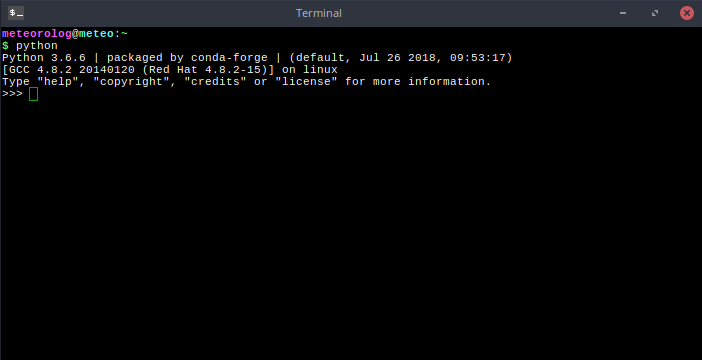
\includegraphics[width=1.\linewidth]{python.png}
\caption*{\textsl{Slika 1. Pokretanje pythona}}
\end{figure}
Uglavnom sve distribucije linuxa dolaze sa instaliranim pythonom, razlika može biti u verziji. Postoje dve verzije pythona, 2.7 čija podrška polako prestaje i novija 3.x (trenutna je 3.6.6). Razlike između ove dve verzije postoje, ali metpy biblioteka koja nama je potrebna podržava obe verzije. Više o razlikama između ove dve verzije pogledajte na \url{https://wiki.python.org/moin/Python2orPython3}. Koja verzija pythona je instalirana možemo proveriti i kucanjem sledećeg koda u terminal:
\begin{lstlisting}
 python --version
 Python 3.6.6
\end{lstlisting}  
U buduće svaki kod će biti vezan za ovu verziju.
\subsection{Izbegavanje problema sa dve verzije}
Kao što sam već spomenuo sve linux distribucija dolaze sa instaliranim pythonom, razlike mogu biti u verziji. Ukoliko vaša linux distribucija ima instaliranu samo verziju 2.7 a vi bi hteli i verziju 3.x, onda treba obratiti pažnju na sledeće. Kod mene, ja koristim MX linux distribuciju baziranu na Debian(stable) verziji, kucanjem u terminalu:
\begin{lstlisting}
 python --version
 Python 3.6.6
\end{lstlisting}  
\begin{figure}[h!]
\centering
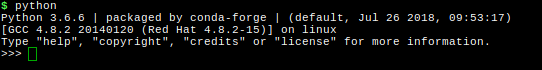
\includegraphics[width=1.\linewidth]{python3.png}
\caption*{\textsl{Slika 2. Pokretanje pythona verzije 3.6.6}}
\end{figure}
prikazuje da je podrazumevana verzija 3.6. Međutim, ukoliko je kod vas instalirana samo verzija 2.7 a vi dodatno instalirante verziju 3.x, može se desiti da će verzija 2.7 i dalje ostati podrazumevana, pa se prilikom kompajliranja može javiti problem. Pošto su kod mene obe vezije, kao podrazumevana verzija je 3.6.6 dok je za pozivanje verzije 2.7 potrebno kucati sledeće:
\begin{lstlisting}
 python2 --version
 Python 2.7.13
\end{lstlisting}
\begin{figure}[h!]
\centering
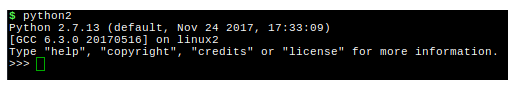
\includegraphics[width=1.\linewidth]{python2.png}
\caption*{\textsl{Slika 3. Pokretanje pythona verzije 2.7}}
\end{figure}
  Kako bi otklonili ovaj problem, u direktorijumu \textsl{/home/user/.bashrc}, koristeći jedna od tekst editora, upišemo sledeću komandu:
\begin{lstlisting}
 alias python=python3
\end{lstlisting}  
Ovom komandom prilikom svakog pozivanja pythona iz terminala kao podrazumevana verzija će biti 3.6.6, što će biti jako bitno u daljem radu.
 \section{Korišćenje biblioteka}
Mnoge python funkcije su sadržane u specijalizovanim bibliotekama, tzv. modulima. Učitavanje modula se postiže naredbom \textsl{import}. Ova mogućnost je pythonu donela popularnost jer postoje monogo modula koji jako pomažu prilikom rada. Python je provo svoju popularnost stekao pri izradi veb programa međutim usavršavanjem podrške za dodtane module otvorilo je vrata pythonu i u drugim oblastima. Moduli poput \textsl{numpy} i \textsl{pandas}, koji se koriste za analizu i vizuelno prikazivanje podataka, su python svrstali uz rame sa ostalim kako komercijalnim programima tako i sa programima otvorenog koda kao što su R, MATLAB, SAS, Stata i ostali. Kada pogledamo da python spada u besplatni programski jezik, njegova popularnost nije slučajnost. Jedan deo ove popularnosti u obradi podataka pripada i laka integracija sa C, C++ i FORTRAN kodom.  
Pošto su moduli jako značajni za python istaći ćemo neke od naznačajnijih. Samo da napomene, sve nabrojane mogućnosti koje pružaju biblioteke je moguće izvesti koristeći isključivo samo Pythonov kod. Prednost biblioteka je u efikasnosti i lakoći kojim se postižu isti rezultati, uz manje utrošenog vremena.  
\subsection{NumPy}
NumPy (\textsl{Numerical Python}) predstavlja fundamentalnu open source Python biblioteku kada su obzir uzmu numerički proračuni. Sadrži matematičke funkcije zadužene za operaciju na podacima, koje se veoma brzo i efikasno izvršavaju. Poziva se komandom :
\begin{lstlisting}
 import numpy as np
\end{lstlisting}
gde \textsl{np} predstavlja skraćenicu od numpy. Kao primer koristićemo funkciju \textsl{np.linspace} kojom se generišu brojevi u zadatom intervalu.  
\begin{figure}[h!]
\centering
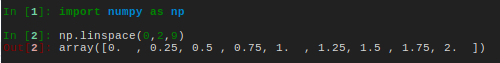
\includegraphics[width=1.\textwidth]{Screenshot.png}
\caption*{\textsl{Slika 4. Pozivanje numpy funkcije np.linspace za generisanje devet brojeva u opsegu od nula do dva. }}
\end{figure}

Za numeričke proračune, nizovi kod NumPy su dosta efikasniji prilikom njihove manipulacije nego bilo koja druga izgrađena struktura unutar Pythona. Instaliranje \textsl{numpy} biblioteke se radi na sledeći način:
\begin{lstlisting}
 conda install numpy
\end{lstlisting}
 Ažuriranje novije verzije se radi na sledeći način:
\begin{lstlisting}[language=Python]
 conda update numpy
\end{lstlisting}
\subsection{Pandas}
Pandas je dizajniran kako bi se ubrzao rad sa strukturiranim ili tabelarnim podacima i kao takav, postao jako moćna i produktivna alatka za analizu podataka. Ono što krasi ovu biblioteku je i velika podrška od strane zajednice, njen aktivna razvoj, odličan rad sa ostalim bibliotekama, izgrađena je na osnovama \textsl{numpy} pa je takođe krasi brzina. Neke od mogućnosti koje pruža ova biblioteka su:
\begin{itemize}
  \item ulaz-izlaz podataka u različitim formatima (csv, txt, SQL...)
  \item indeksiranje, sortiranje, rangiranje
  \item čišćenje podataka 
  \item grupisanje
  \item vizuelizacija
\end{itemize}
Sačinjenja je od dve strukture podataka, \textsl{dataframe} i \textsl{series}.  \textsl{Series} predstavljaju jednodimenzioni objekat sačinjen od tabele sa vrednostima i njihovim indeksima. 
\begin{figure}[h!]
\centering
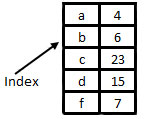
\includegraphics[width=0.4\textwidth]{pandas-series.jpg}
\caption*{\textsl{Slika 5. Pandas series }}
\end{figure}
\textsl{Dataframe} predstavlja tabelarnu strukturu podataka, definisanih u dve ili više dimenzije.  Sačinjen je od tri osnovne komponente: podataka, indeksa, kolona. 
\begin{figure}[h!]
\centering
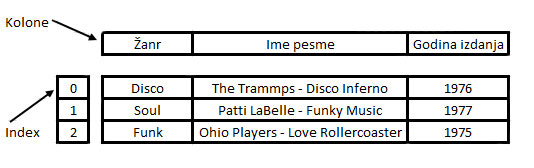
\includegraphics[width=0.8\textwidth]{pandas-dataframe.jpg}
\caption*{\textsl{Slika 6. Pandas dataframe }}
\end{figure}
Skraćenjica za \textsl{pandas} je \textsl{pd}, poziva se korišćenjem komande:
\begin{lstlisting}[language=Python]
 import pandas as pd 
\end{lstlisting}
Kao primer uzeću mogućnost ubacivanja podataka iz \textsl{.csv} dokumenta, to se radi na sledeći način:
\begin{lstlisting}[language=Python]
 df = pd.csv_read('ime_dokumenta.csv')
\end{lstlisting}
Instaliranje pandas biblioteke:
\begin{lstlisting}
 conda install pandas
\end{lstlisting}
\subsection{Matplotlib}
Najviše korišćena i najstarija biblioteka koja se koristi za vizuelno predstavljanje podataka. U kombinaciji sa \textsl{numpy} i \textsl{pandas} čine jako moćne alate, koji se mogu nositi sa komercijalnim i dosta skupim alatima kao što su \textsl{Matlab} i \textsl{Mathematica}. Mana ove biblioteke je potreba za pisanjem većeg broja linija koda kako bi se dobila naprednija vizuelizacija podataka. 
Potreba za povećanim kvalitetom vizuelizacije, nastale su savremenije biblioteke koje se u većoj ili manjoj meri oslanjaju na \textsl{matplotlib}. Jedna od takvih biblioteka je \textsl{seaborn} čiji je fokus na  atraktivnijoj izradi statističkih grafika.  \textsl{Seaborn} se potpuno oslanja na \textsl{matplotlib}.  Naveo bih još i \textsl{bokeh} i \textsl{altair} koje nisu zavisne od \textsl{matplotlib}, a takođe se koriste za vizuelizaciju podataka.
\subsection{MetPy}
Metpy predstavlja kolekciju alata u Pythonu za pregled, vizuilizaciju i proračuna meteoroloških podataka. Paket je nastao od strane \textsl{Unidata} udruženja, koja se bavi izradom alata za naučne svrhe. MetPy paket sadrži dosta opcija, koristi se za vizelizaciju radarskih slika, rad sa netCDF podacima,vizuelizaciju radio-sondažnih merenja, vizuelizaciju meteoroloških podataka i ostalo. Mi ćemo koristi ovu biblioteku u svrhu interpolacije polja temperature. Za instaliranje MetPy u terminal kucamo:
\begin{lstlisting}
 conda install -c -conda-forge metpy
\end{lstlisting}
Instaliranjem ovog paketa dobijamo razne alate, nama će najviše značiti mogućnost interpolacije za polje temperature kao i negove vizuelizacije. Za vizuilizaciju se koristi \textsl{Cartopy}, Pythonov paket za crtanje mapa.


\end{document}
